\section{Linear regression}

The goal of regression is to approximate a function $f(x)$ that maps input $x$ to a continuous output $t$ from a dataset $\mathcal{D}$: 
\[\mathcal{D}=\left\{ \left\langle x,t \right\rangle \right\} \implies t=f(x)\]
Here, $x$ is a vector. 
To perform regression, we assume the existence of a function capable of performing this mapping.
The key components of constructing a linear regression problem include:
\begin{itemize}
    \item The method used to model the function $f$ (the hypothesis space). 
    \item The evaluation criteria for the approximation (the loss function).
    \item The optimization process for optimizing the model.
\end{itemize}

In linear regression, the function $f$ is modeled using linear functions. 
This choice is motivated by several factors:
\begin{itemize}
    \item Linear models are easily interpretable, making them suitable for explanation.
    \item Linear regression problems can be solved analytically, allowing for efficient computation.
    \item Linear functions can be extended to model nonlinear relationships.
    \item More sophisticated methods often build upon or incorporate elements of linear regression.
\end{itemize}

\paragraph*{Hypothesis space}
In mathematical terms, the approximation $y$ can be defined as: 
\[y(\textbf{x},\textbf{w})=w_0+\sum_{j=1}^{D-1}w_j x_j=\textbf{w}^T\textbf{x}\]
Here, $\textbf{x} = \left( 1,x_1,\dots,x_{D-1} \right)$ is a vector, and $w_0$ is called the bias parameter.
It's important to note that the output $y$ is a scalar value. 

In a two-dimensional space, our hypothesis space will be the set of all points in the plane $(w_0,w_1)$. 
The coordinates of each point will correspond to a line in the $\left( \textbf{x}, y \right)$ space.

\paragraph*{Loss function}
A commonly used error loss function for the linear regression problem is the sum of squared errors (SSE), defined as:
\[L(\textbf{w})=\dfrac{1}{2}\sum_{n=1}^{N}\left( y(x_n, \textbf{w})-t_n \right)^2\]
This sum is also referred to as the residual sum of squares (RSS) and can be expressed as the sum of squared residual errors:
\[RSS(\textbf{w})=\left\lVert \boldsymbol{\epsilon}^2_2 \right\rVert = \sum_{i=1}^{N}\epsilon^2_i \]
This formulation of the loss function allows for obtaining a closed-form optimization solution.

\paragraph*{Optimization}
For linear models, a closed-form optimization of the RSS, known as least squares, begins with the matrix representation of the loss function:
\[L(\textbf{w})=\dfrac{1}{2}RSS(\textbf{w})=\dfrac{1}{2}\left( \textbf{t}-\boldsymbol{\Phi}_{\textbf{w}} \right)^T\left( \textbf{t}-\boldsymbol{\Phi}_{\textbf{w}} \right)\]
Here, $\boldsymbol{\Phi}=\begin{bmatrix} \phi(x_1) & \dots & \phi(x_N)\end{bmatrix}^T$ and $\textbf{t}=\begin{bmatrix}t_1 & \dots & t_n\end{bmatrix}^T$.
To find the optimal $\textbf{w}$, we compute the first derivative of $L(\textbf{w})$ and set it to zero:
\[\widehat{\textbf{w}}_{OLS}=\left( \boldsymbol{\Phi}^T\boldsymbol{\Phi}\right)^{-1}\boldsymbol{\Phi}^T\textbf{t}\]
However, the inversion of the matrix $\boldsymbol{\Phi}^T\boldsymbol{\Phi}^{-1}$ can be computationally expensive, especially for large datasets, with a complexity of $O(nm^2+m^3)$, assuming the matrix is non-singular (invertible). 

To mitigate this, stochastic gradient descent (SGD) can be employed. 
The algorithm known as least mean squares (LMS) uses the following update rule:
\[L(\textbf{x})=\sum_nL(x_n)\]
Expanding this, we get:
\begin{align*}
    \textbf{w}^{(n+1)}  &= \textbf{w}^{(n)}-\alpha^{(n)}\nabla L(x_n) \\
                        &= \textbf{w}^{(n)}-\alpha^{(n)}\left( \textbf{w}^{(n)^T}\phi(\textbf{x}_n)-t_n \right)\phi(\textbf{x}_n)
\end{align*}
Here, $\alpha$ is the learning rate, and convergence is guaranteed if $\sum_{n=0}^{\infty}=+\infty$ and $\sum_{n=0}^{\infty}=\alpha^{(n)^2}<+\infty$.

If the regression problem involves multiple outputs, meaning that $\textbf{t}$ is not a scalar, we can solve each regression problem independently.
However, we can still use the same set of basis functions.
The solution for the weight vectors for all outputs can be expressed as:
\[\widehat{\textbf{W}}=\left( \boldsymbol{\Phi}^T\boldsymbol{\Phi}\right)^{-1}\boldsymbol{\Phi}^T\textbf{T}\]
Here, each column of matrix $\textbf{T}$ and $\widehat{\textbf{W}}$ corresponds to the target vector and the weight vector for each output, respectively.
This solution can be easily decoupled for each output $k$: 
\[\widehat{\textbf{w}}_k=\left( \boldsymbol{\Phi}^T\boldsymbol{\Phi}\right)^{-1}\boldsymbol{\Phi}^T\textbf{t}_k\]
An advantage of this approach is that $\left( \boldsymbol{\Phi}^T\boldsymbol{\Phi}\right)^{-1}$ only needs to be computed once, regardless of the number of outputs.

\subsection{Basis function}
While a linear combination of input variables may not always suffice to model data, we can still construct a regression model that is linear in its parameters. 
This can be achieved by defining a model using non-linear basis functions, expressed as:
\[y(\textbf{x},\textbf{w})=w_0+\sum_{j=1}^{M-1}w_j \phi_j(\textbf{x})=\textbf{w}^T\boldsymbol{\phi}(\textbf{x})\]
Here, the components of the vector  $\boldsymbol{\phi}(\textbf{x})=\left( 1,\phi_1(\textbf{x}),\dots,\phi_{M-1}(\textbf{x}) \right)^T$  are referred to as features.
These features allow for a more flexible representation of the input data, enabling the model to capture non-linear relationships between the input variables and the output.
\begin{example}
    Let's reconsider a set of data regarding individuals' weight and height, along with their completion times for a one-kilometer run:
    \begin{table}[H]
        \centering
        \begin{tabular}{c|c|c}
        \textbf{Height (cm)} & \textbf{Weight (kg)} & \textbf{Completion time (s)} \\ \hline
        180                  & 70                   & 180                          \\
        184                  & 80                   & 220                          \\
        174                  & 60                   & 170                         
        \end{tabular}
    \end{table}
    We can model this problem using a dummy variable and introduce the Body Mass Index (BMI) as a new feature:
    \begin{table}[H]
        \centering
        \begin{tabular}{c|c|c|c|c}
        \textbf{Dummy variable} & \textbf{Height (cm)} & \textbf{Weight (kg)} & \textbf{BMI} & \textbf{Completion time (s)} \\ \hline
        $x_0$                   & $x_1$                & $x_2$                & $x_3$        & $t$                          \\
        1                       & 180                  & 70                   & 21           & 180                          \\
        1                       & 184                  & 80                   & 23           & 220                          \\
        1                       & 174                  & 60                   & 20           & 170                         
        \end{tabular}
    \end{table}
    Here, the dummy variable $x_0$ is always initialized to one.
    Now, we have the option to retain or discard the weight and height variables, considering only the BMI values for analysis.
\end{example}
The most commonly used basis functions in regression are:
\begin{itemize}
    \item \textit{Polynomial}: 
        \[\phi_j(x)=x^j\]
    \item \textit{Gaussian}:
        \[\phi_j(x)=\exp \left( -\dfrac{\left( x-\mu_j \right)^2}{2 \sigma^2} \right) \]
    \item \textit{Sigmoidal}: 
        \[\phi_j(x)=\dfrac{1}{1+\exp\left(\dfrac{\mu_j-x}{\sigma}\right)}\]
\end{itemize}
Here, the constant $\mu_j$ is referred to as a hyperparameter, as its value needs to be determined through experimentation and depends on the user's experience.

\begin{figure}[H]
    \centering
    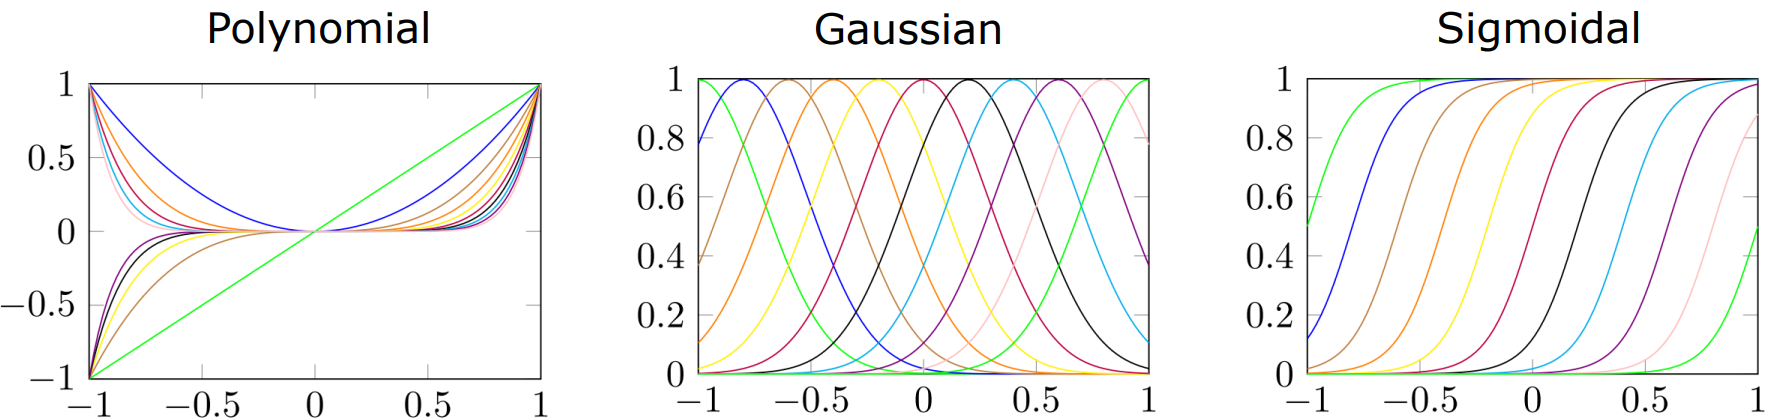
\includegraphics[width=0.75\linewidth]{images/basis.png}
    \caption{Some possible basis functions shapes}
\end{figure}

It's noteworthy that the Gaussian basis function allows for a local approximation by omitting values that are close to zero.
This approach enables capturing the relationship between the input and output in a reduced input space area.
As we move away from the mean, approaching zero, the values become negligible.

\subsection{Regularization}
A function can achieve a better approximation by increasing the degree of the polynomial used in the regression.
\begin{example}
    Consider a function generating a set of points with some noise:
    \begin{figure}[H]
        \centering
        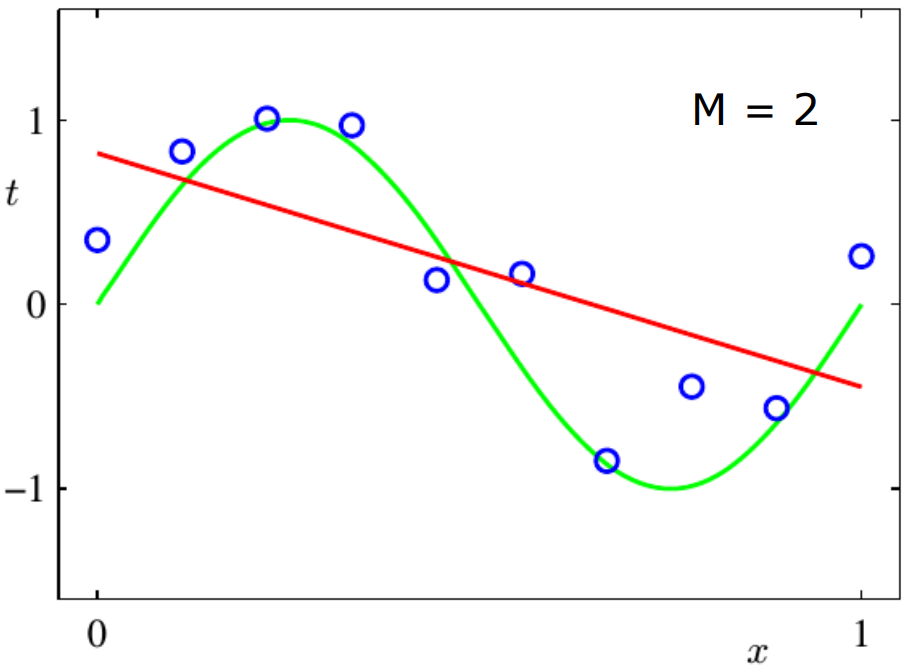
\includegraphics[width=0.25\linewidth]{images/reg.png}
    \end{figure}
    Using a second-order polynomial instead of a linear one provides a better approximation:
    \begin{figure}[H]
        \centering
        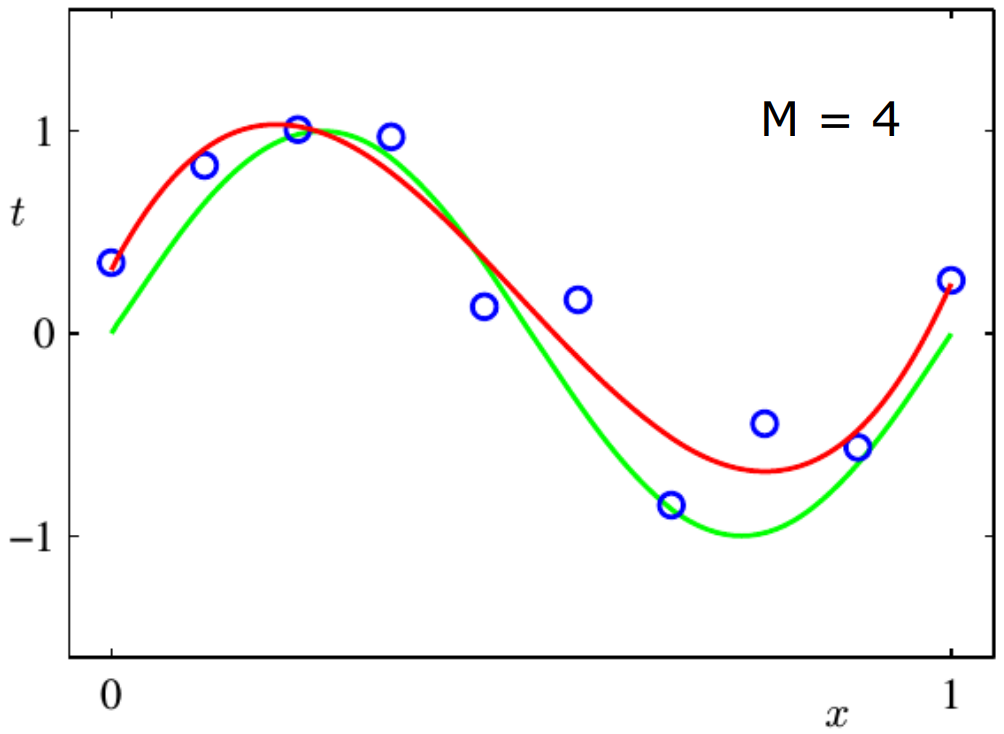
\includegraphics[width=0.25\linewidth]{images/reg1.png}
    \end{figure}
    Further improving the approximation can be achieved with a higher-degree polynomial (e.g., ninth grade):
    \begin{figure}[H]
        \centering
        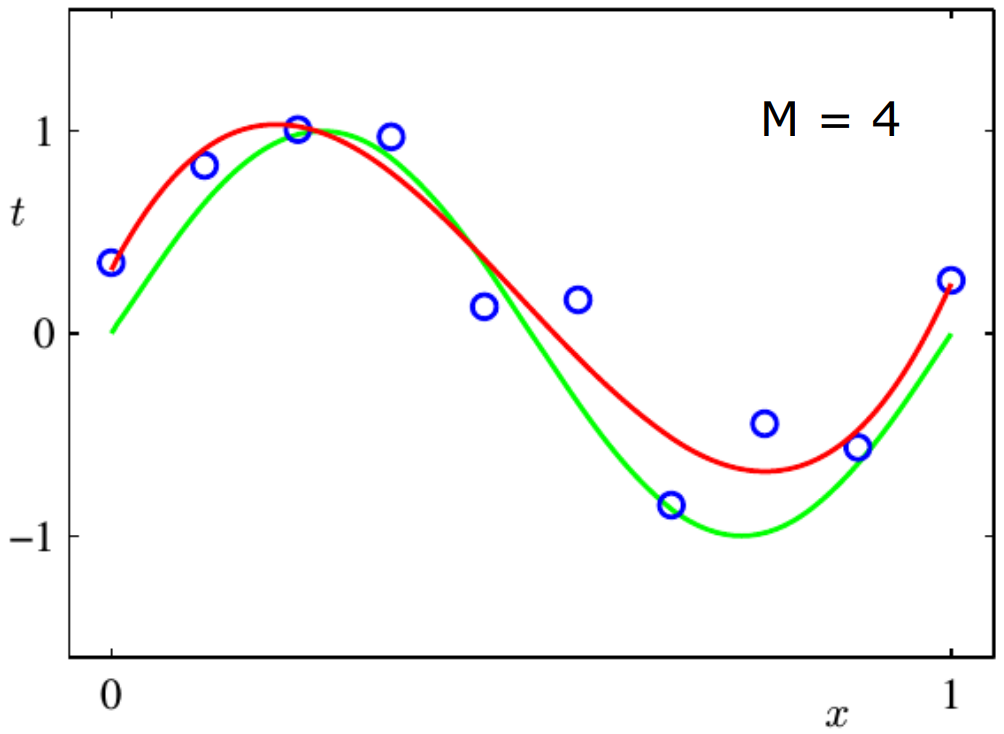
\includegraphics[width=0.25\linewidth]{images/reg1.png}
    \end{figure}
\end{example}
However, increasing the polynomial degree also increases the complexity of the model parameters.
To address this complexity, adjustments are needed in the loss function:
\[L(\textbf{w})=L_D(\textbf{w})+\lambda L_W(\textbf{w})\]
Here, $L_D(\textbf{w})$ represents the usual loss function, $L_W(\textbf{w})$ reflects model complexity (a hyperparameter), and $\lambda$ is the regularization coefficient.
$L_W(\textbf{w})$ can be tailored using ridge regression or lasso methods.

\paragraph*{Ridge regression}
In ridge regression, the regularization term $L_W(\textbf{w})$ is defined as:
\[L_W(\textbf{w})=\dfrac{1}{2}\textbf{w}^T\textbf{w}=\dfrac{1}{2}\left\lVert \textbf{w} \right\rVert_2^2 \]
Thus, the overall loss function becomes:
\[L(\textbf{w})=\dfrac{1}{2}\sum_{i=1}^N \left( t_i-\textbf{w}^T\phi(x_i) \right)^2 + \dfrac{\lambda}{2}\left\lVert \textbf{w} \right\rVert_2^2\]
Despite the regularization term, the loss function remains quadratic with respect to $w$, allowing for closed-form optimization:
\[\widehat{\textbf{w}}_{ridge}=\left( \lambda\textbf{I}+\boldsymbol{\Phi}^T \boldsymbol{\Phi} \right)^{-1}\boldsymbol{\Phi}^T\text{t}\]
The term $\lambda\textbf{I}$ is crucial in solving the singularity problem, as it transforms a non-singular matrix into a singular one with an appropriate choice of $\lambda$. 

\paragraph*{Lasso}
Another common regularization method is lasso, where the regularization term $L_W(\textbf{w})$ is defined as:
\[L_W(\textbf{w})=\dfrac{1}{2}\left\lVert \textbf{w} \right\rVert_1=\dfrac{1}{2}\sum_{j=0}^{M-1}\left\lvert w_j \right\rvert\]
Thus, the overall loss function becomes:
\[L(\textbf{w})=\dfrac{1}{2}\sum_{i=1}^N \left( t_i-\textbf{w}^T\phi(x_i) \right)^2 + \dfrac{\lambda}{2}\left\lVert \textbf{w} \right\rVert_1\]
In this case, closed-form optimization is not possible. 
However, lasso typically leads to sparse regression models: when the regularization coefficient $\lambda$ is large enough, some components of $\widehat{\textbf{w}}$ become equal to zero.
Regularization can be seen as equivalent to minimizing  $L_D(\textbf{w})$ subject to the constraint:
\[\sum_{j=0}^{M-1}\left\lvert w_j \right\rvert \leq \eta\]